\documentclass[UTF8]{ctexart}
\usepackage{amsmath,amssymb}
\usepackage{mathrsfs}
\usepackage{graphicx}
\usepackage{subfigure}
\usepackage{geometry}
\title{\heiti 引力波作业报告}
\author{\kaishu 刘苏明}
\date{\today}
\geometry{a4paper, left=3.18cm, right = 3.18cm, bottom = 2.54cm, top = 2.54cm}
\begin{document}
\maketitle
\section{数据分析}
从网站[https://www.gw-openscience.org/events/GW150914/]可以获取Living和Hanford的引力波探测数据。
\begin{figure}[!htbp]
	\centering
	\subfigure[未修正的引力波波形]{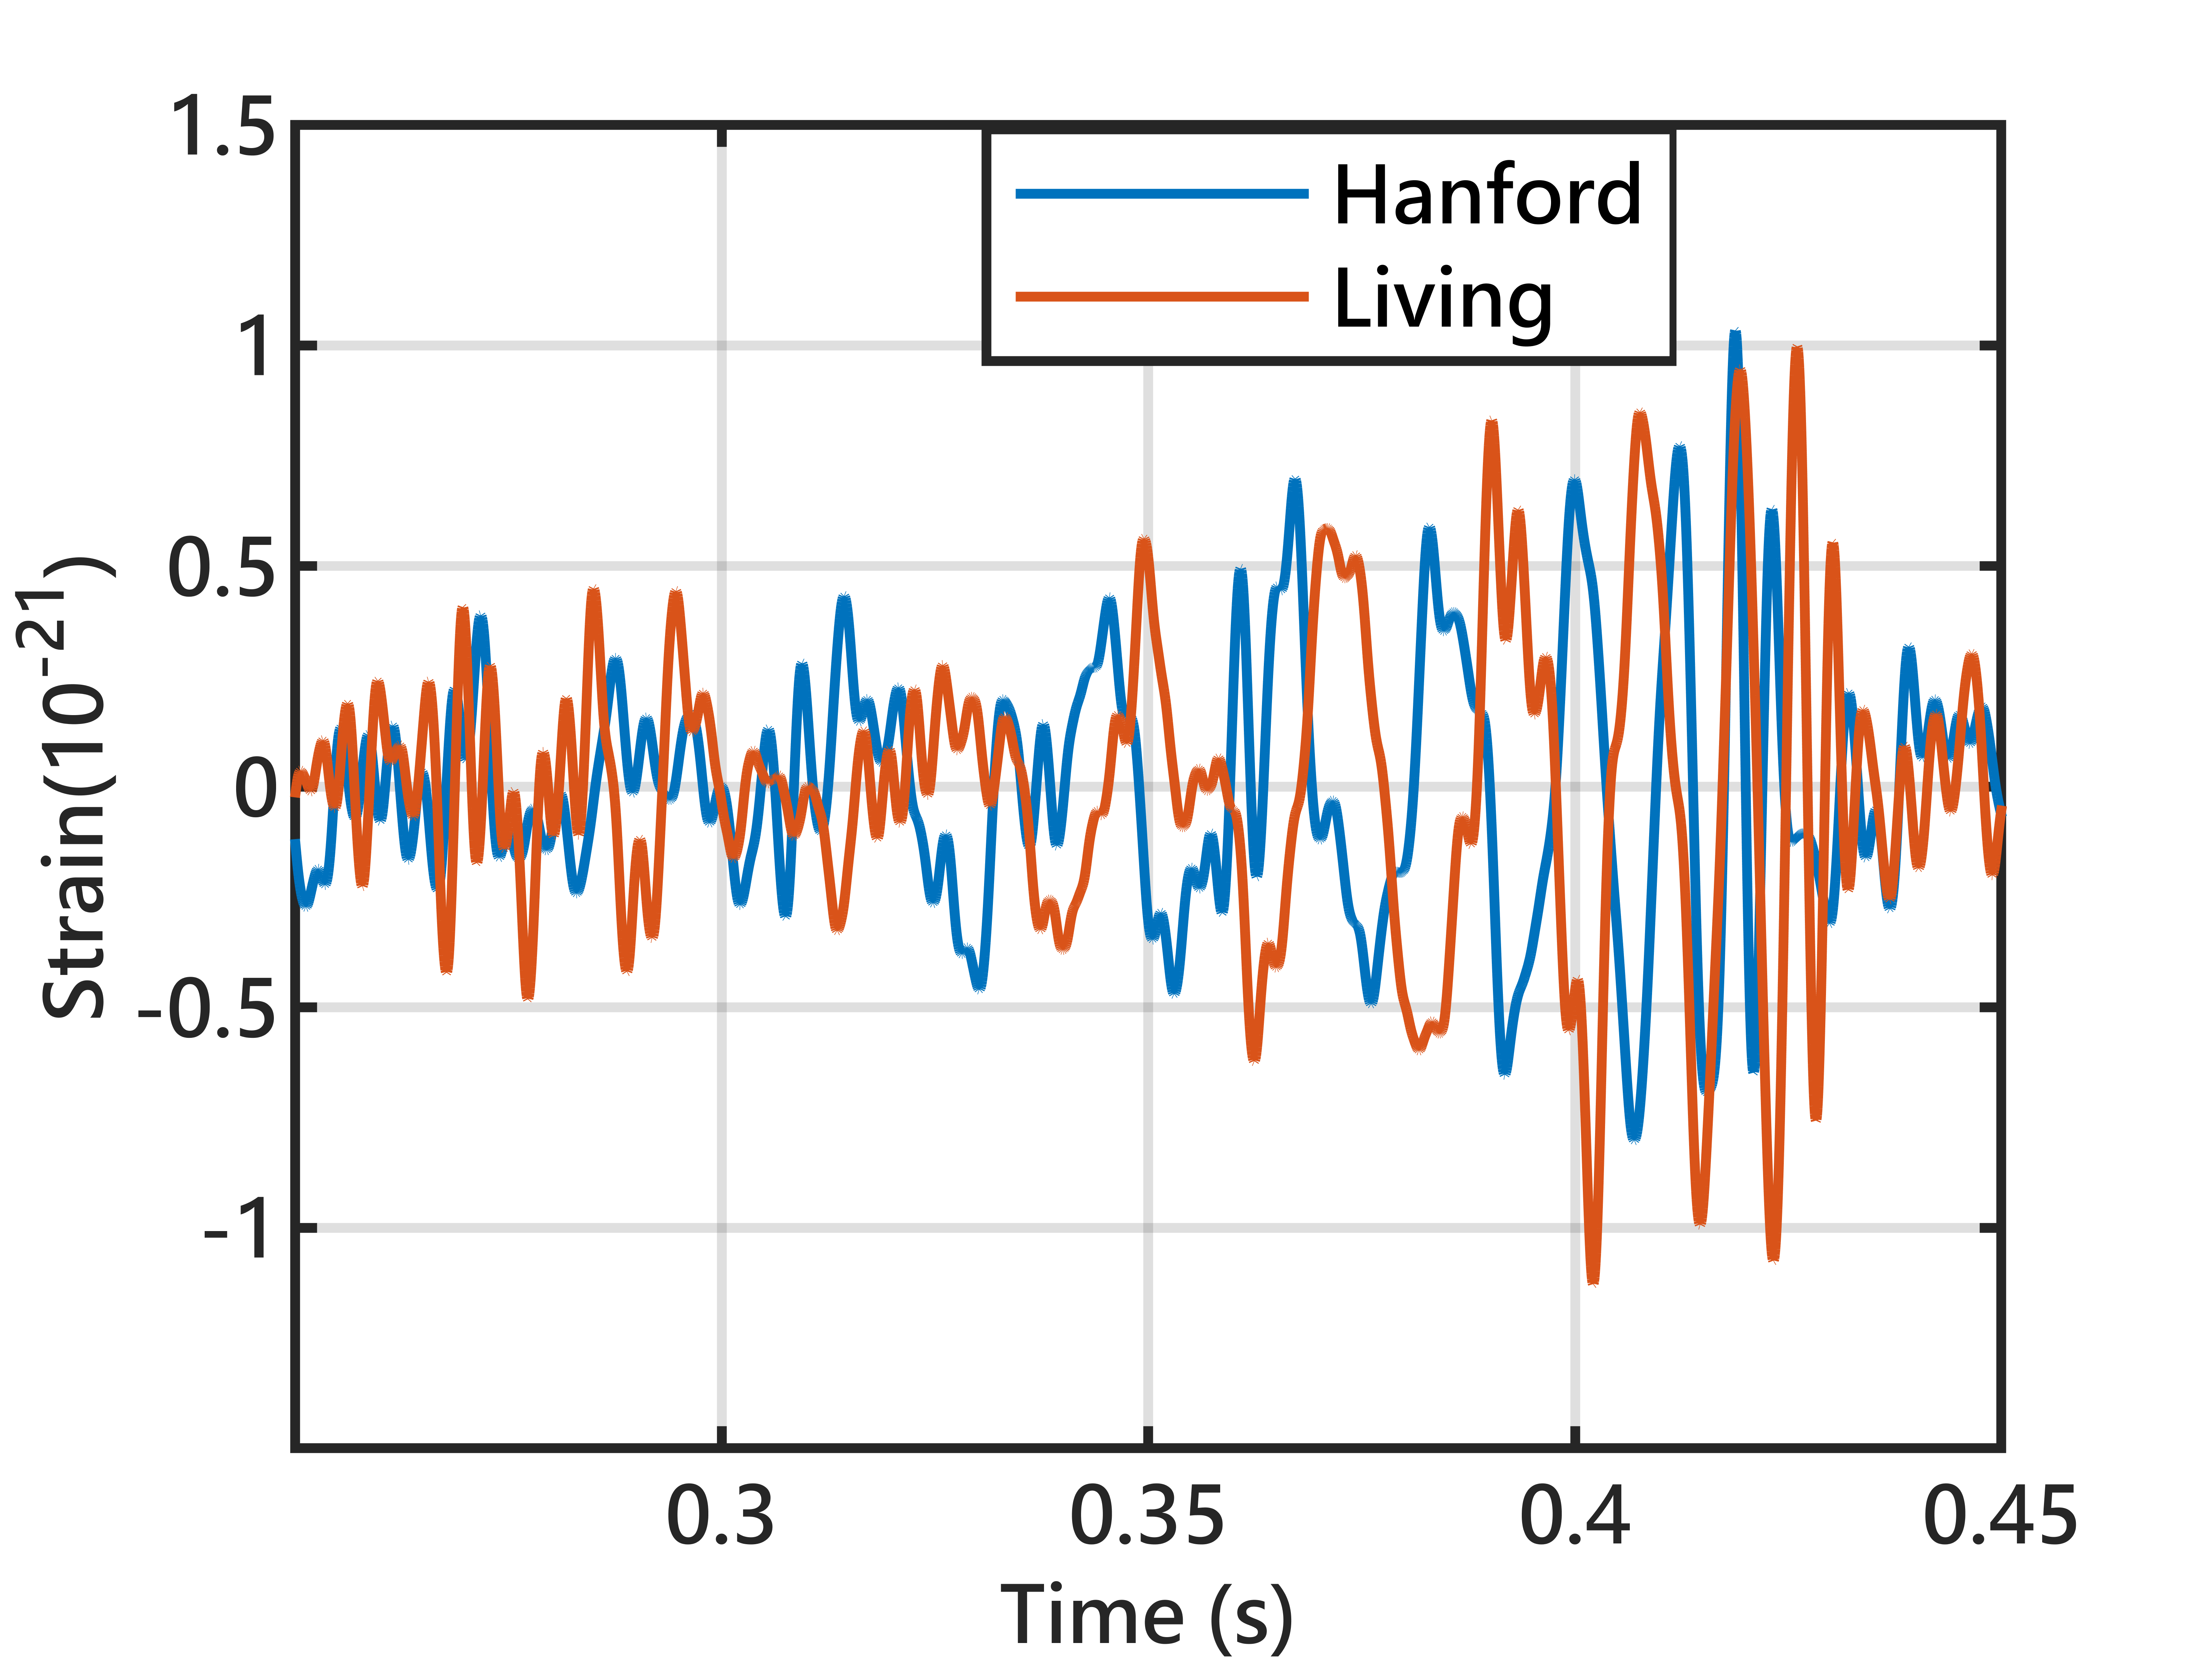
\includegraphics[width = 0.45\hsize]{未修正的引力波数据.png}}
	\subfigure[修正后的引力波波形]{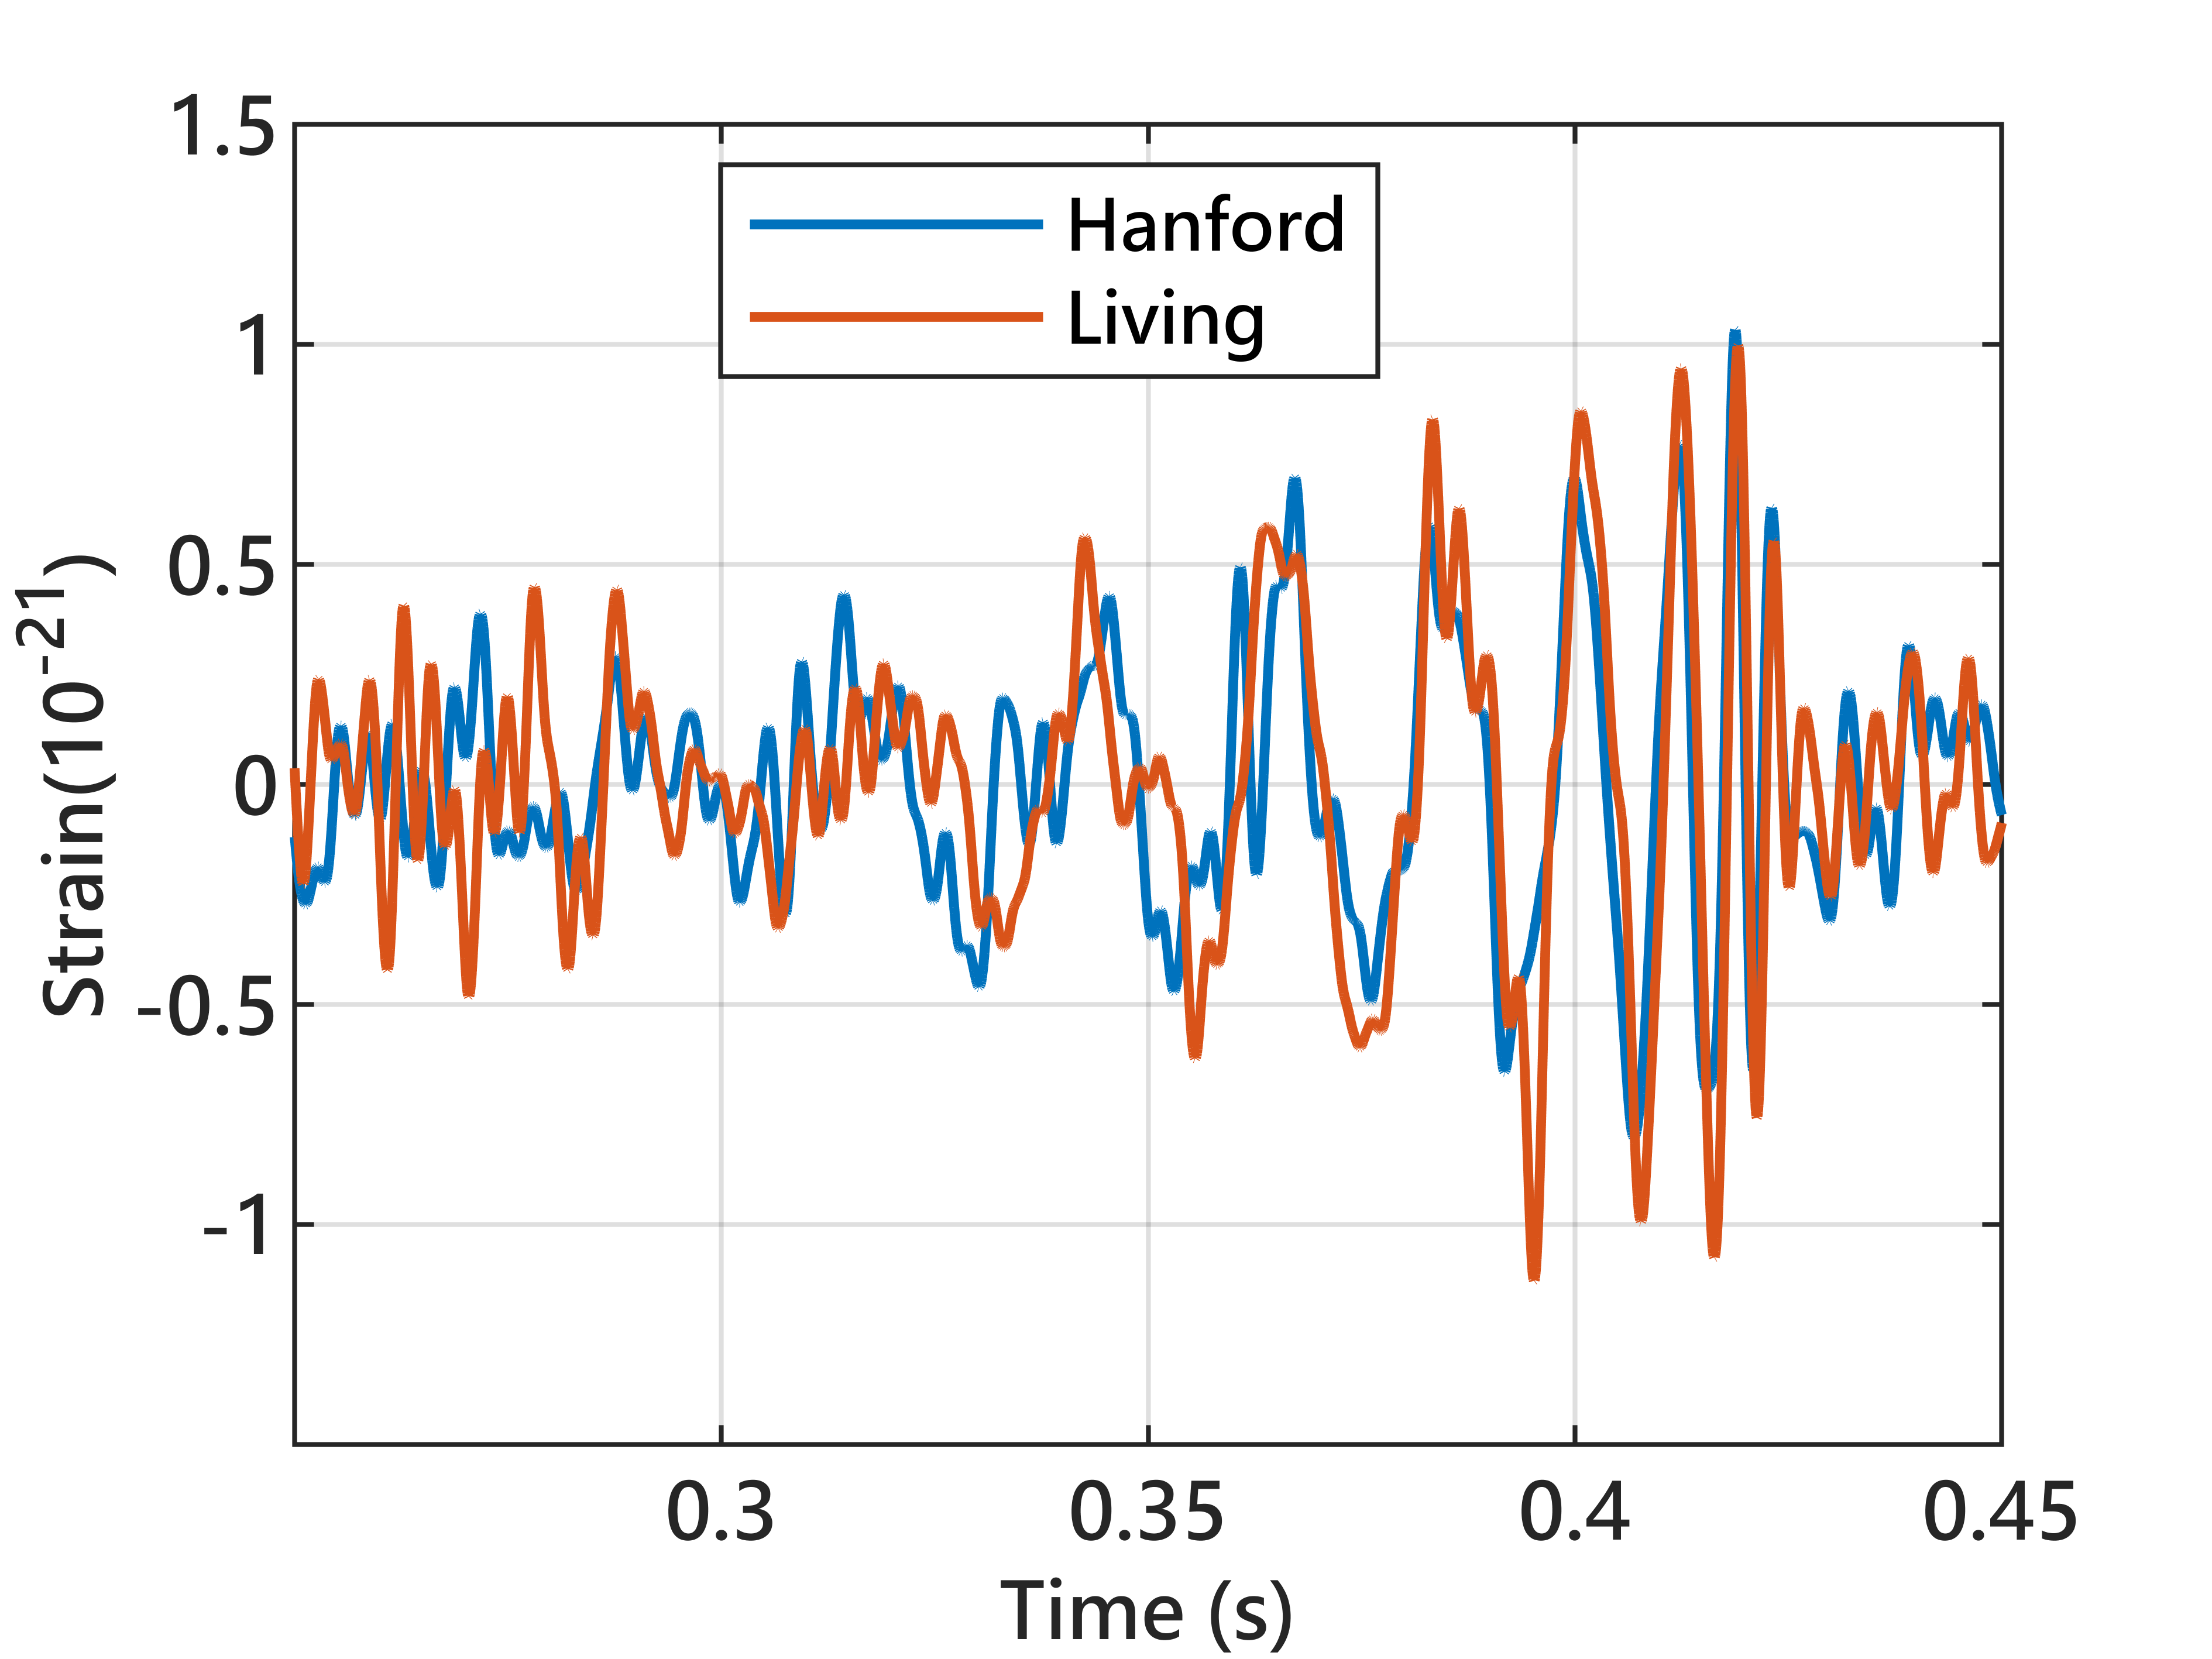
\includegraphics[width = 0.45\hsize]{引力波.png}}
	\caption{引力波波形}
\end{figure}

LIGO Hanford和Livingston探测器在UTC时间为2015年9月14日9:50:45左右探测到了编号为GW150914的引力波。为了更值地看到引力波波形,原始数据经过30Hz-350Hz的滤波器,因为这是探测器灵敏度最高的频率带。同时应用带阻滤波器消除仪器产生的高频谱噪声。经过处理后得到图1(a)的图像。 这时Living和Hanford的波形还存在较大差异, 因为Living和Hanford的地理位置不同,Living首先探测到引力波信号,比Hanford早6.9ms,而且两者的探测方向相反。 所以图1(a)的数据需要修正。 修正后的引力波波形如图1(b)所示。

\begin{figure}[!htbp]
	\centering
	\subfigure[Hanford 的时频图]{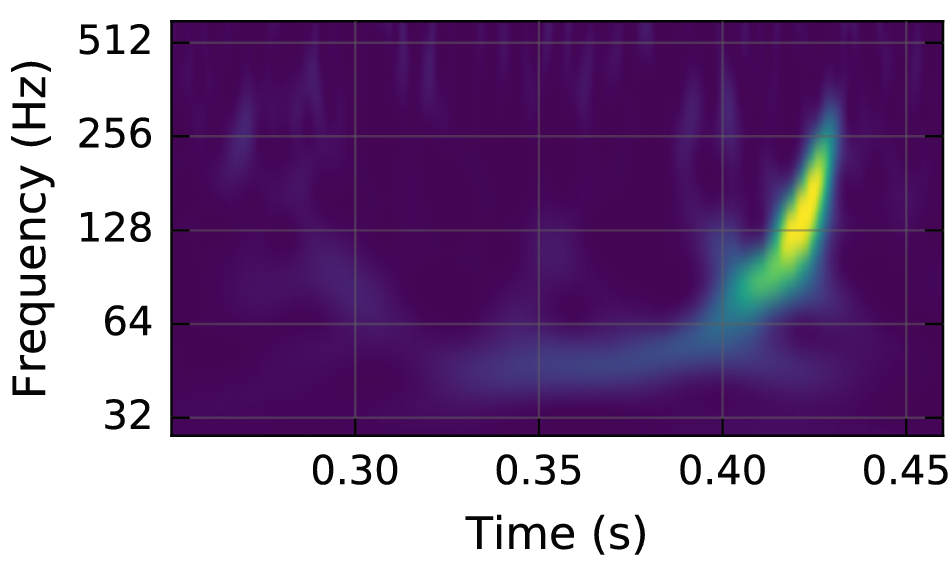
\includegraphics[width = 0.45\hsize]{fig1-freqtime-H.png}}
	\subfigure[Living 的时频图]{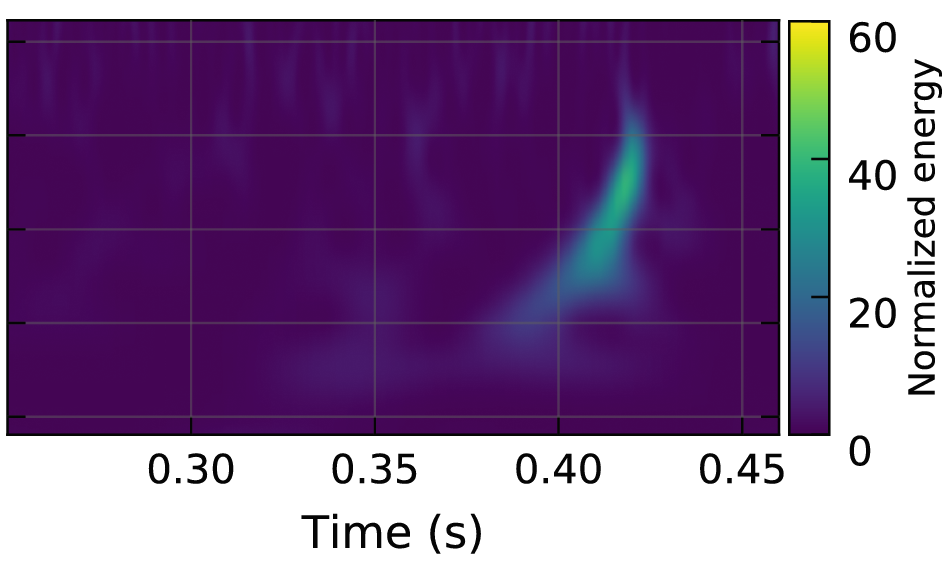
\includegraphics[width = 0.45\hsize]{fig1-freqtime-L.png}}
	\caption{时频图}
\end{figure}
图2表示Hanford和Living的引力波能量随时间和频率变化的图像。从图中可以看出,随着时间和频率的增大,引力波能量也在增大。从0.3s开始,引力波周期减小,所以频率开始增大。在0.42s左右,能量迅速下降,频率趋于稳定。最后,引力波的瞬时频率高于200Hz。整个过程持续了大概0.15s。

广义相对论中,质量在加速的情况下会产生引力波。由于波形表现出了至少八个振荡周期,所以存在一个或多个质量在振荡。引力波频率和能量的增大也表示在这段时间里引力波源的振荡频率也在增大。在引力波频率和能量都在增大时,天体的轨道运动只有一个合理的解释:引力波向外辐射能量,它产生了天体运动唯一的阻力,使得两个天体在不断靠近,频率不断增大且放大了引力波辐射的能量。

我们将证明,随观测到的频率演化唯一合理的解释是,该系统由两个黑洞组成,它们相互环绕,绕后合并在一起。

\textbf{确定能量最大时对应的频率}$f_{\rm GW}|_{\rm max}$ : 在证明时,一个非常重要的物理量是能量最大时的频率值。 利用图1的峰值或者图2的最亮点附近的过零点,我们保守地计算处该值
\begin{equation}
f_{\rm GW}|_{\rm max} \sim 150{\rm Hz},
\end{equation}
因此我们可以把引力波源的轨道运动解释为,天体做轨道运动时,轨道角频率不超过某个值
\begin{equation}
\omega_{\rm Kep}|_{\rm max}=\frac{2\pi f_{\rm GW}|_{\rm max}}{2} = 2\pi \times 75 {\rm Hz}
\end{equation}

\textbf{确定引力波源的质量量级}:爱因斯坦发现无迹质量四极矩为$Q_{ij}$的系统在视界距离为$d_L$产生的引力波形变$h$为
\begin{equation}
h_{ij}=\frac{2G}{c^4d_L}\frac{{\rm d^2}Q_{ij}}{{\rm d}t^2}
\end{equation}
引力波辐射能量的速率可以由四极质量公式推出
\begin{equation}
\label{E4}
\begin{aligned} \frac{\mathrm{d} E_{\mathrm{GW}}}{\mathrm{d} t}=& \frac{c^{3}}{16 \pi G} \iint|\dot{h}|^{2} \mathrm{d} S=\frac{1}{5} \frac{G}{c^{5}} \sum_{i, j=1}^{3} \frac{\mathrm{d}^{3} Q_{i j}}{\mathrm{d} t^{3}} \frac{\mathrm{d}^{3} Q_{i j}}{\mathrm{d} t^{3}} \\ & \text { where }|\dot{h}|^{2}=\sum_{i, j=1}^{3} \frac{\mathrm{d} h_{i j}}{\mathrm{d} t} \frac{\mathrm{d} h_{i j}}{\mathrm{d} t} \end{aligned}
\end{equation}
其积分区域为半径为$d_L$的球。方程(\ref{E4})表示当轨道天体的速度远小于光速且引力波形变也不大时的轨道能量损失速率。在频率达到$f_{\rm GW}|_{\rm max}$前,我们会一直使用它。

对于一个双天体系统,我们使用$m_1, m_2$表示两天体的质量,使用$M=m_1+m_2$表示天体的总质量,$\mu = m_1m_2/M$表示减少的质量,质量系数为$q=m_1/m_2$,假设$m_1\geq m_2$即$q\geq 1$.我们可以定义chirp mass 为$\mathscr{M}$来表示双天体引力波源系统向外辐射引力波的表达式
\begin{equation}
\mathscr{M} = \frac{(m_1m_2)^{3/5}}{(m_1+m_2)^{1/5}}
\end{equation}

使用牛顿运动定律,万有引力定律和爱因斯坦的引力波光度四极方程,导出了一个简单的公式,把引力波的频率与频率导数和chirp mass联系起来。
\begin{equation}
\label{E6}
\mathscr{M}=\frac{c^{3}}{G}\left(\left(\frac{5}{96}\right)^{3} \pi^{-8}\left(f_{\mathrm{GW}}\right)^{-11}\left(\dot{f}_{\mathrm{CW}}\right)^{3}\right)^{1 / 5}
\end{equation}
只要牛顿运动定律有效,这个公式就有效。

所以我们可以通过观测数据使用引力波的频率和频率导数计算任意时刻的chirp mass。当然,$\mathscr{M}$的确切值是多少并不重要,为了简单起见,我们设$\mathscr{M}=30M_\odot$。

chirp mass在$f_{\rm GW}|_{\rm max}<150{\rm Hz}$会保持不变,这样就给解释轨道运动提供了有力的支持。引力波应变的能量随频率增加也支持这样的解释,且计算中这些公式的假设是适用的:1. 双星系统的速度远小于光速;2. 轨道运动的半径在不断减少;3. 使用开普勒定律来描述周期。

chirp mass 还可以换一种计算方法
\begin{equation}
f_{\mathrm{GW}}^{-8 / 3}(t)=\frac{(8 \pi)^{8 / 3}}{5}\left(\frac{G \mathscr{M}}{c^{3}}\right)^{5 / 3}\left(t_{c}-t\right)
\end{equation}
这个方程不包含频率的导数,所以可以直接通过应变数据的过零点的时间间隔来计算$\mathscr{M}$.常数$t_c$是合并时刻。图3更直观的展示了这个现象。

\section{证明天体是致密的}
为了简化计算,我们设两个天体的质量相等,$m_1=m_2$。也就是说$m_1=m_2=2^{1/5}\mathscr{M}=35M_\odot,M=m_1+m_2=70M_\odot$。假设天体不存在自旋而且它们的轨道符合开普勒定律,在合并前都保持着圆轨道。

根据万有引力定律,合并时刻的天体距离为
\begin{equation}
R = \left(\frac{\rm GM}{\omega^2_{\rm Kep|max}}\right)^{1/3} = 350{\rm km}
\end{equation}
和天体的半径向相比,这个数字相当小。白矮星的半径有1000km。密度最大的天体是中子星,半径只有10km。如果观测到的中子星,在这种距离下它们不会合并但是中子星的质量最大只有$3M_\odot$。所以中子星也不是我们的目标天体。

在我们的简化计算中,天体质量为$m_1=m_2=M_\odot$.每个天体半径为施瓦茨席尔德半径$r = 103{\rm km}$,如图3所示。
\begin{figure}[!htbp]
	\centering
	\subfigure{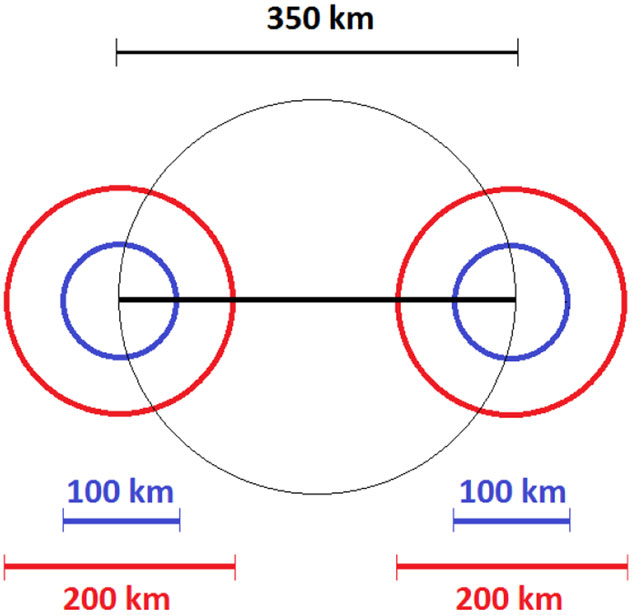
\includegraphics[height =0.4\hsize]{figure4.png}}
	\caption{最小天体距离和施瓦茨席尔德半径的图示}
\end{figure}

为了定量描述天体间的靠近程度,我们定义了紧密度系数$\mathscr{R}=R/(r_1+r_2)$。所以我们的双向系统的致密度系数为$\mathscr{R}=350{\rm km}/206{\rm km} \sim 1.7$.和其它著名的开普勒轨道系统相比,水星与太阳的紧密度系数达到$\mathscr{R}\sim 2\times 10^7$,两个中子星构成的系统在合并前紧密度系数在2和5之间。

所以,从开普勒定律和牛顿运动定律出发,GW150914在到达合并时刻时其紧密度系数达到黑洞量级,足以证明其密度非常大。

\section{假设的影响}
在第2节,我们计算出了引力波源是黑洞,但是它有三个前提,圆形轨道、质量相同、无自旋。本节会讨论这些假设如何影响结论。
\subsection{轨道偏心率}
非圆轨道,偏心率$e>0$,$R$不再是天体的距离,而是轨道半长轴的长度。那么天体轨道距离存在最大值和最小值$(1-e)R<r_{sep}<R$。同时亮度(luminosity)也需要基于偏心率作出调整,但是这只对大偏心率的轨道运动有意义。如果目标轨道的偏心率比较大,信号会在高振幅和低振幅峰值振荡。但这种现象并不存在,正如前文所说,幅值是单调递增。这是因为引力波带走的角动量导致轨道的旋转速度比收缩速度快很多。所以轨道偏心率对结论没有影响。
\subsection{质量不相等}
致密度系数$\mathscr{R}$随质量系数$q$的增大而减少。我们使用chirp mass和质量系数来表示天体质量。$m_1=\mathscr{M}(1+q)^{1/5}q^{2/5},m_2 = \mathscr{M}(1+q)^{1/5}q^{-3/5},M=m_1+m_2=\mathscr{M}(1+q)^{6/5}q^{-3/5}$.致密度系数可以表示为
\begin{equation}
\begin{aligned}
\mathscr{R} &=\frac{R}{r_{\text {Schwarz }}(M)}=\frac{c^{2}}{2\left(\left.\omega_{\text {Kep }}\right|_{\max } G M\right)^{2 / 3}} \\
&=\frac{c^{2}}{2\left(\left.\pi f_{\text {GW }}\right|_{\max } G \mathscr{M}\right)^{2 / 3}} \frac{q^{2 / 5}}{(1+q)^{4 / 5}} \approx \frac{3.0 q^{2 / 5}}{(1+q)^{4 / 5}}
\end{aligned}
\end{equation}

如图4所示,致密度系数$R$随质量系数增大而减小。所以,当chirp mass和轨道角频率确定时,天体质量不相等会导致天体密度更大。那么目标天体只能是黑洞。

\begin{figure}[!htbp]
	\centering
	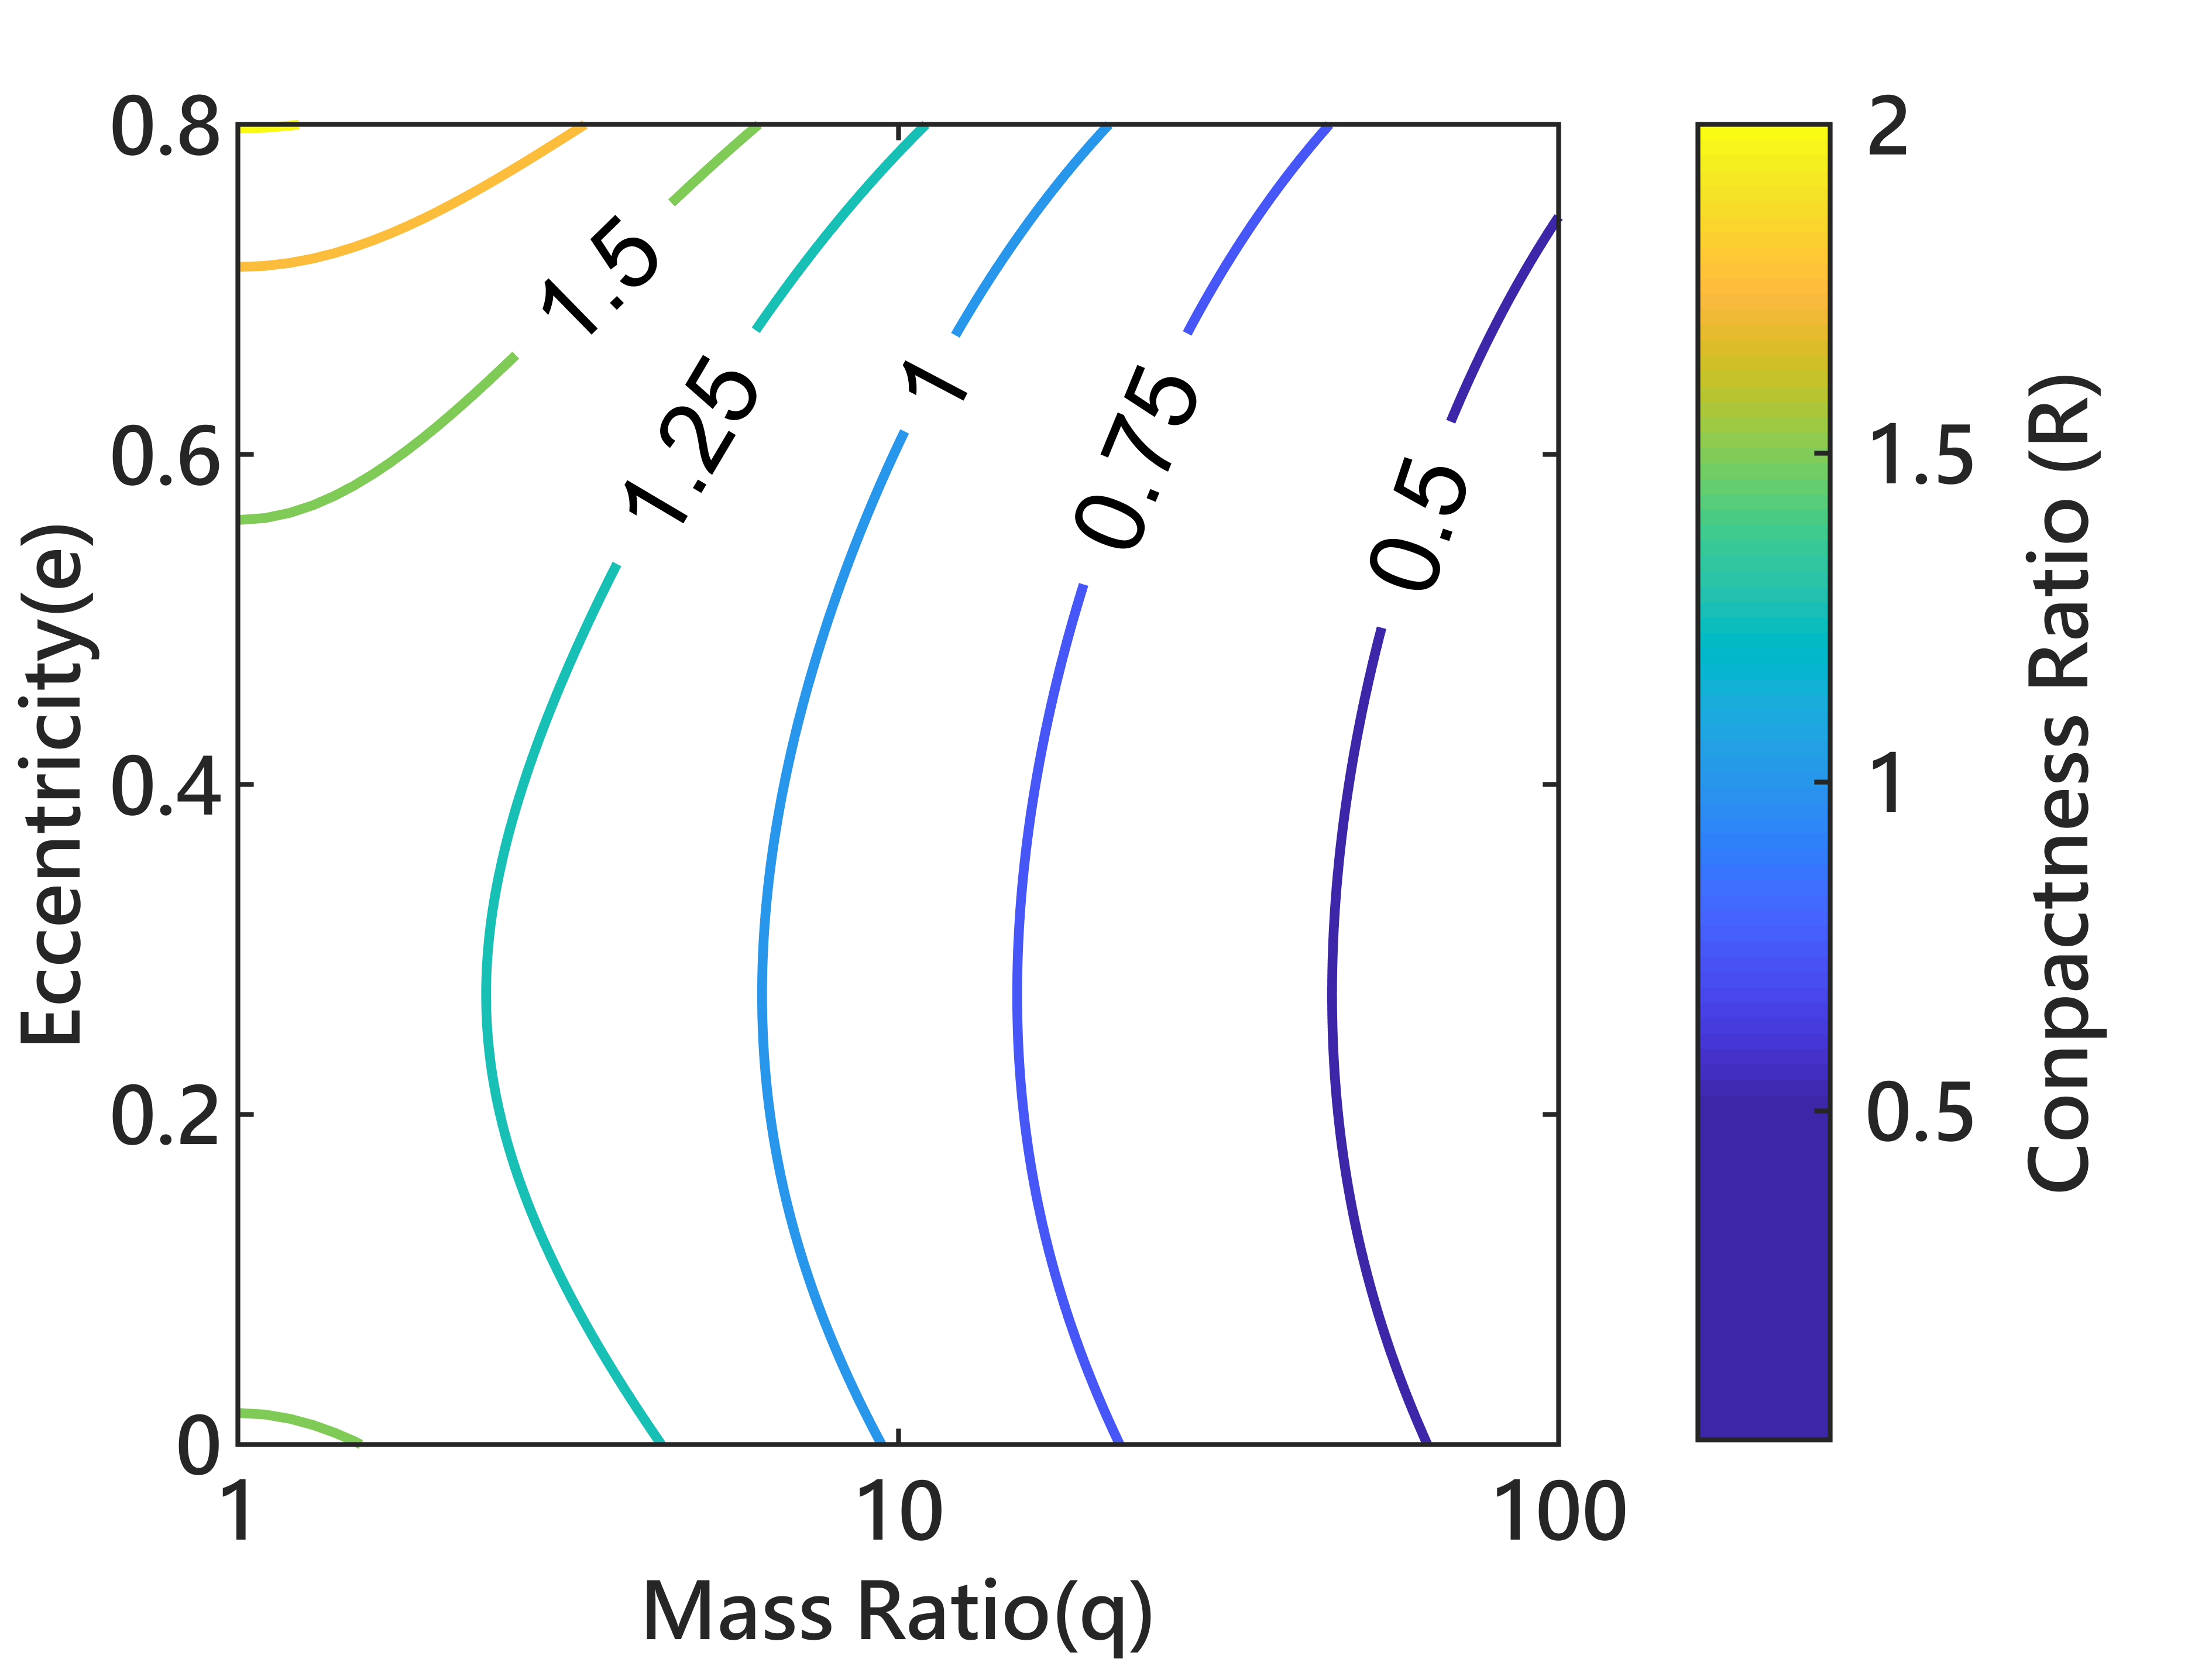
\includegraphics{figure-5.png}
	\caption{致密度系数R随离心率e和质量系数q变化}
\end{figure}

\subsection{天体自旋}
质量为m,角动量为S的天体,我们定义旋转参数为
\begin{equation}
\chi = \frac{c}{G}\frac{S}{m^2}
\end{equation}
天体的自旋会影响天体的引力半径和轨道运动。对于非黑洞天体,无自旋的最小半径是施瓦茨席尔德半径。当天体存在角动量时,比如$\chi=1$,天体的最小引力半径会是施瓦茨席尔德半径的一半。$r_{\rm EK}(m) =\frac{1}{2}r_{\rm Schwarz}(m)=Gm/c^2 $,它与天体质量成正比。对于非黑洞天体,最小半径和为
\begin{equation}
\begin{aligned}
r_{\mathrm{EK}}\left(m_{1}\right)+r_{\mathrm{EK}}\left(m_{2}\right) &=\frac{1}{2} r_{\mathrm{Schwarz}}(M) \\
&=\frac{G M}{c^{2}} \approx 1.5\left(\frac{M}{\mathrm{M}_{\odot}}\right) \mathrm{km}
\end{aligned}
\end{equation}

存在自旋现象的天体的致密度系数要比没有自旋的大得多。$\mathscr{M}\simeq3.4$是无自旋的两倍。所以存在自旋现象的天体的密度要更大。
\begin{equation}
\begin{aligned}
\mathscr{R} &=\frac{r_{\mathrm{sep}}(M)}{r_{\mathrm{EK}}(M)} \leq \frac{R(M)}{r_{\mathrm{EK}}(M)}=\frac{c^{2}}{\left(G M \omega_{\mathrm{Kep}}\right)^{2 / 3}} \\
& \leq \frac{c^{2}}{\left(2^{6 / 5} G \mathscr{M} \omega_{\mathrm{Kep}}\right)^{2 / 3}} \\
& = \frac{c^2}{(2^{6/5}\pi\mathscr{M}f_{\rm GW}|_{\rm max})^{2/3}} \simeq 3.4\end{aligned}
\end{equation}

所以无论有没有自旋和相等的质量,结论都不变:目标天体是黑洞。

\section{距离和光度(luminosity)}
一些基本的物理参数可以用来估计引力波的光度和波源与我们的距离以及辐射的总能量。引力波的振幅$h$随着距离$d_L$的增加而下降,$h\propto1/d_L$.图1表示,我们测得的应变峰值大约为$10^{-21}$。当距离减小十倍时,峰值增大十倍。但是靠近波源中心时,峰值不会成比例的增大,因为引力波的非线性效应会非常明显。这种情况下,我们估算出一个粗略的数量级上界
\begin{equation}
d_L<10^{21}\times200{\rm km}\sim6{\rm Gpc}
\end{equation}

我们还可以通过光度来更准确的估计距离,因为等质量的天体辐射的引力波光度的峰值与质量无关。根据四极公式,光度$L\sim \frac{G}{c^5}M^2r^4\omega^6$,在最后的合并时刻有$\omega\sim c/t,r\sim GM/c^2,M\omega\sim c^3/G$。我们可以得到Plank光度。

\begin{equation}
L\sim L_{\rm Planck}=c^5/G=3.6\times10^{52}W
\end{equation}

\begin{equation}
\label{A}
\frac{dE}{dt}=\frac{32}{5}\frac{G}{c^5}\mu^2r^4\omega^6
\end{equation}
然而,根据公式(\ref{A}),光度的系数应该为$\frac{32}{5}({\mu}/{M})^2$,同时对天体半径缩小成施瓦西半径的情况进行分析可以得到$M\sim \frac{1}{6}c^2r_{\rm ISCO}/G$和$\omega r\sim 0.5c$。把这些情况考虑进来,$L$的修正系数应有$0.2\times 10^{-3}$。方程(\ref{E4})可以把距离为$d_L$引的力波光度与应变$h$联系起来。
\begin{equation}
L=\frac{{\rm d}E_{\rm GW}}{{\rm d}t}=\frac{c^3}{16\pi G}\iint|\dot{h}|^2{\rm d}S\sim\frac{c^3d_L^2}{4G}|\dot{h}|^2\sim\frac{c^5}{4G}\left(\frac{\omega_{\rm GW}d_Lh}{c}\right)^2
\end{equation}
所以我们可以得到
\begin{equation}
\frac{L_{\rm peak}}{L_{\rm Planck}} \equiv \frac{L|_{\rm max}}{L_{\rm Planck}}\sim 0.2\times 10^{-3}\sim \left(\frac{\omega_{\rm GW}d_Lh|_{\rm max}}{c}\right)^2 
\end{equation}

我们在峰值达到最大时估计随应变值变化的距离为
\begin{equation}
d_L\sim 45{\rm Gpc}\left(\frac{\rm Hz}{f_{\rm GW|_{\rm max}}}\right) \left(\frac{10^{-21}}{h|_{\rm max}}\right)
\end{equation}
对于GW150914而言,$d_L\sim 300{\rm Mpc}$。

\begin{equation}
\label{A2}
E_{\rm orb} = -\frac{GM\mu}{2r}
\end{equation}
利用方程(\ref{A2}),我们可以估计引力波的辐射总能量。从初始距离时$E_{\rm orb}^i\to0$到距离为$r$时,代入$m_1\sim m_2\sim35M_\odot,r\sim R = 350{\rm km}$
\begin{equation}
E_{\rm GW}=E_{\rm orb}^i-E_{\rm orb}^f = 0-\left(-\frac{GM\mu}{2R}\right)\sim3M_\odot c^2
\end{equation}
这是总能量的最低估计值。

这个能量非常大。在100亿年的生命周期中,太阳预计会将不到1\%的能量转化为光和辐射。GW150914不仅会辐射了将近300倍太阳一生辐射的能量,其在峰值的光度也比太阳大出了22个数量级。
\section{总结}
使用一些基本的物理参数理解观测的GW150914应变数据,我们可以得到许多更深层次的结论。这些结论表明引力波源是一对在合并前非常接近的互旋黑洞。合并后稳定形成一个黑洞。我们还可以通过一些简单的参数求出这个波原离为我们的距离和基本信息。

本文只是一个科普文章,其方法并不通用,可能只适合于与GW150914相似的信号。希望本文可以为读者提供理解引力波探测的起点。
\end{document}